\documentclass{article}
\usepackage{import}
\usepackage[utf8]{inputenc}
\usepackage{amsmath}
\usepackage{amssymb}
\usepackage{mathtools}
\usepackage{graphicx}
\usepackage{tabularx}
\usepackage{float}
\usepackage{subfig}
\usepackage{lscape} 
\usepackage{hyperref}
\usepackage{setspace}
\usepackage{booktabs}
\usepackage[authoryear]{natbib}
\usepackage{lmodern}
\usepackage[T1]{fontenc}
\usepackage[bottom]{footmisc}
\newcommand{\indep}{\perp \!\!\! \perp}
\usepackage[nolist]{acronym}
\newcommand\headercell[1]{%
   \smash[b]{\begin{tabular}[t]{@{}c@{}} #1 \end{tabular}}}
\usepackage[a4paper,top=3cm,bottom=2cm,left=3cm,right=3cm,marginparwidth=1.75cm]{geometry}
\usepackage{xcolor}%
\definecolor{webbrown}{rgb}{.6,0,0}
\usepackage{hyperref}%
\hypersetup{%
  breaklinks = true,%
  colorlinks = true,%
  anchorcolor = webbrown,%
  citecolor = webbrown,%
  filecolor = webbrown,%
  linkcolor = webbrown,%
  menucolor = webbrown,%
  urlcolor= webbrown,%
  citebordercolor= 1 0 0,%
  menubordercolor=1 0 0,%
  urlbordercolor=1 0 0,%
  runbordercolor=1 0 0,}
\usepackage{cleveref}

\usepackage{setspace}
\usepackage{enumitem}
\setstretch{1.5} %% set line spacing

\begin{acronym}
  \acro{CI}{confidence interval}
  \acro{RCT}{randomized controlled trial}
  \acro{IV}{instrumental variable}
  \acro{LATE}{local average treatment effect}
  \acro{ATE}{average treatment effect}
  \acro{OLS}{ordinary least squares}
  \acro{RD}{regression discontinuity}
  \acro{MTE}{marginal treatment effect}
  \acro{ATT}{average treatment effect on the treated}
\end{acronym}

\graphicspath{ {../../output/figures/} }

% Wrap table notes
\usepackage{booktabs}
\newcommand{\tabnotes}[2]{\bottomrule \multicolumn{#1}{@{}p{0.70\linewidth}@{}}{\footnotesize #2 }\end{tabular}\end{table}}

\floatplacement{figure}{H}
\floatplacement{table}{H}

\usepackage[toc,page]{appendix}


\title{College Enrollment and Earnings:
\texorpdfstring{\\}{} Examining the Impact of Two Federal Drug Acts}
\author{Ray Huang\thanks{Contact:
    \href{mailto:ray_huang@brown.edu}{ray\_huang@brown.edu}.
     I thank Peter Hull at Brown University for serving as my advisor and for providing me with fantastic feedback. I would also like to thank Alison Lodermeier and Francesco Ferlenga.}
     \\Brown University, Honors Thesis}

\date{\today}

\begin{document}

\maketitle

\begin{abstract}
\noindent (aspirational abstract) I examine the impact of two federal drug acts on college enrollments and earnings among black males by using a variety of counterfactual groups. The Anti-Drug Act of 1986 transformed the formerly rehabilitation-focused justice system into a punitive one, imposed sentencing minimums and disparities. The Fair Sentencing Act of 2010 undid many of these policies. I construct estimates of the impact of these two acts on black males aged 18-24 using three unique counterfactual groups: 1) white males, 2) black females, and 3) black men aged 28-34. I also leverage the variation between high and low drug arrest states. I estimate that the Anti-Drug Act of 1986 resulted in a change in college enrollment rates between XX and XX and a change in earnings between XX and XX. For this subpopulation, this implies estimates of economic returns to education ranging from XX to XX.

\end{abstract}

\clearpage

\section*{Introduction}

Anti-Drug Act of 1986:
\begin{itemize}[itemsep=0.05mm, parsep=0pt]
  \item Created minimum sentencing laws re possession of many drugs. 
  \item Crack/powdered cocaine was particularly relevant (significantly harder rules on crack, which was cheaper and used by minorities much more, 100-1 ratio)
  \item The law led to an increase in the average time imprisoned for drug crimes from 22 months to 33 months (Shewan)
\end{itemize}


Fair Sentencing Act of 2010:
\begin{itemize}[itemsep=0.05mm, parsep=0pt]
  \item Reduced the disparity between the amount of crack cocaine and powder cocaine needed to trigger certain federal criminal penalties from a 100:1 weight ratio to an 18:1 weight ratio 
  \item Elimated minimum sentencing for crack cocaine 
  \item Congressional Budget Office has estimated that implementing the Fair Sentencing Act of 2010 will reduce the prison population by 1,550 person-years over the time period from 2011–2015, creating a monetary savings of \$42 million during that period 
\end{itemize}

Existing literature:
\begin{itemize}[itemsep=0.05mm, parsep=0pt]
  \item The Labor Market Consequences of Incarceration- Western, Kling, Weiman (2016)
  \item Juvenile Incarceration, Human Capital, and Future Crime: Evidence from Randomly Assigned Judges - Aizer, Doyle (2015)
  \item Evan Rose papers: The Impact of Incarceration on Employment and Earnings, etc
\end{itemize}


\section*{Data}

\begin{itemize}[itemsep=0.05mm, parsep=0pt]
  \item CPS October supplement
  \item UCR from ICPSR (missing data problem, many counties failed to report arrest rates for the relevant crimes)
  \item ACS
\end{itemize}

\section*{Empirical/Econometric Methods, Hypotheses tested}


\textbf{Counterfactual groups}
\begin{itemize}[itemsep=0.05mm, parsep=0pt]
  \item Black males vs white males
  \begin{itemize}
    \item Identifying assumption: absent of the Anti-Drug Abuse Act of 1986, black and white male educational outcomes would have trended similarly.
  \end{itemize}
  \item Black males vs black females
  \item Black males aged 18-24 vs black males aged 28-34 at the time of the act
  \item High vs low drug use
\end{itemize}

\textbf{Empirical tools:}
\begin{itemize}[itemsep=0.05mm, parsep=0pt]
  \item DiD / DDD / Event study.
  \item \begin{itemize}
    \item Using Roth's pretrend \& honest did suggestions
  \end{itemize}
  \item DDIV
\end{itemize}

%%%%%%%%%%%%%%%%%%%%%%%%BIB%%%%%%%%%%%%%%%%%%%%%%%%%%%

\clearpage
\nocite{*}
\singlespacing
\bibliographystyle{jpe}
\bibliography{citations.bib}

%%%%%%%%%%%%%%%%%%%%%%%%FIGURES%%%%%%%%%%%%%%%%%%%%%%%%%%%
a
\clearpage

Note: all figures are limited to ages 18-24 inclusive.

\begin{center}
  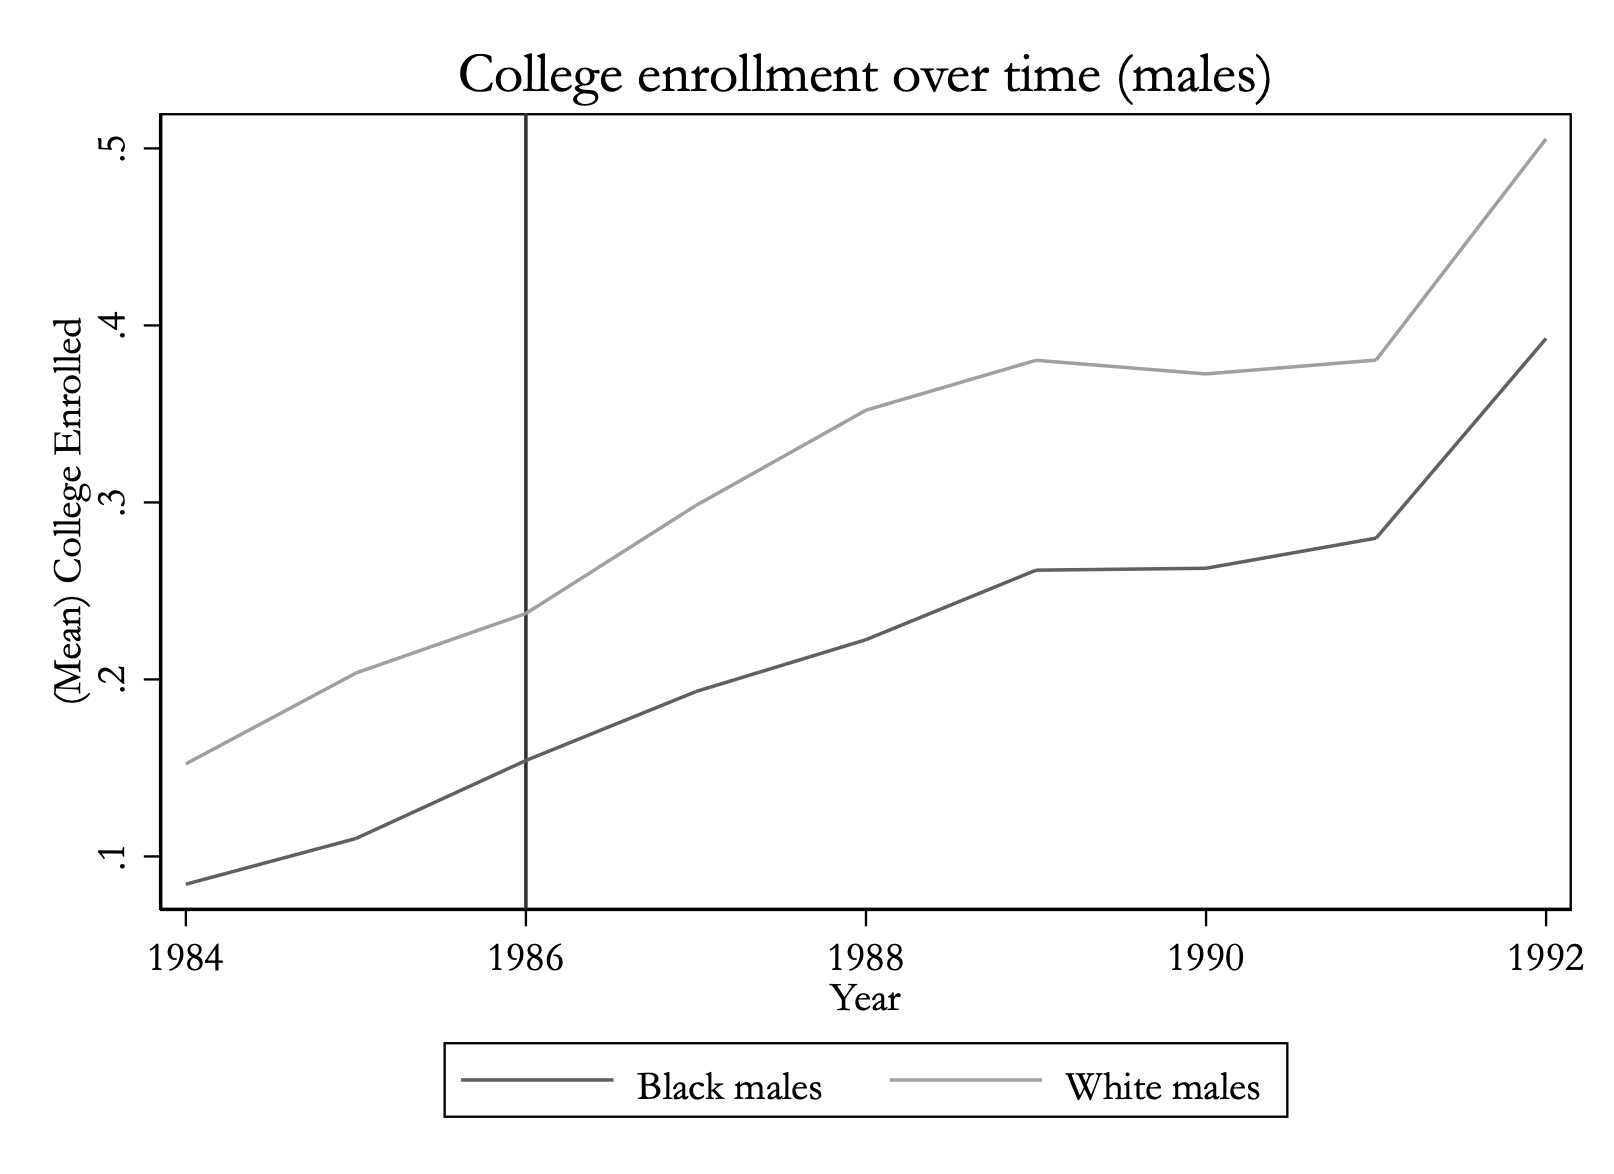
\includegraphics[width=.4\textwidth]{pretrends/1986/college_enroll_byrace_1986.png}
  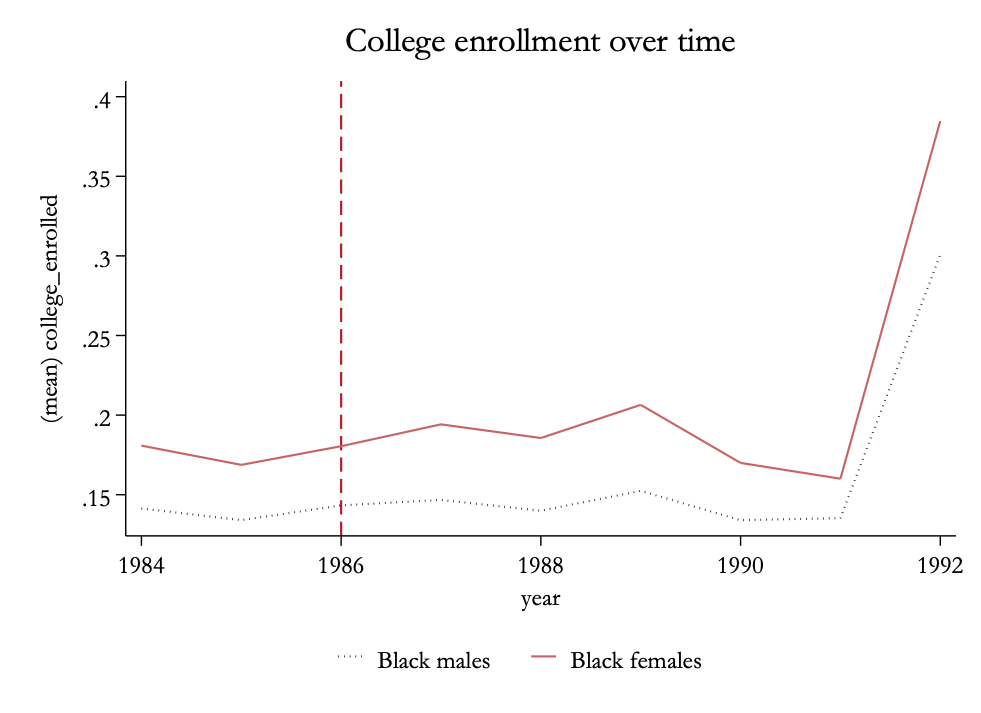
\includegraphics[width=.4\textwidth]{pretrends/1986/college_enroll_bysex_1986.png}
  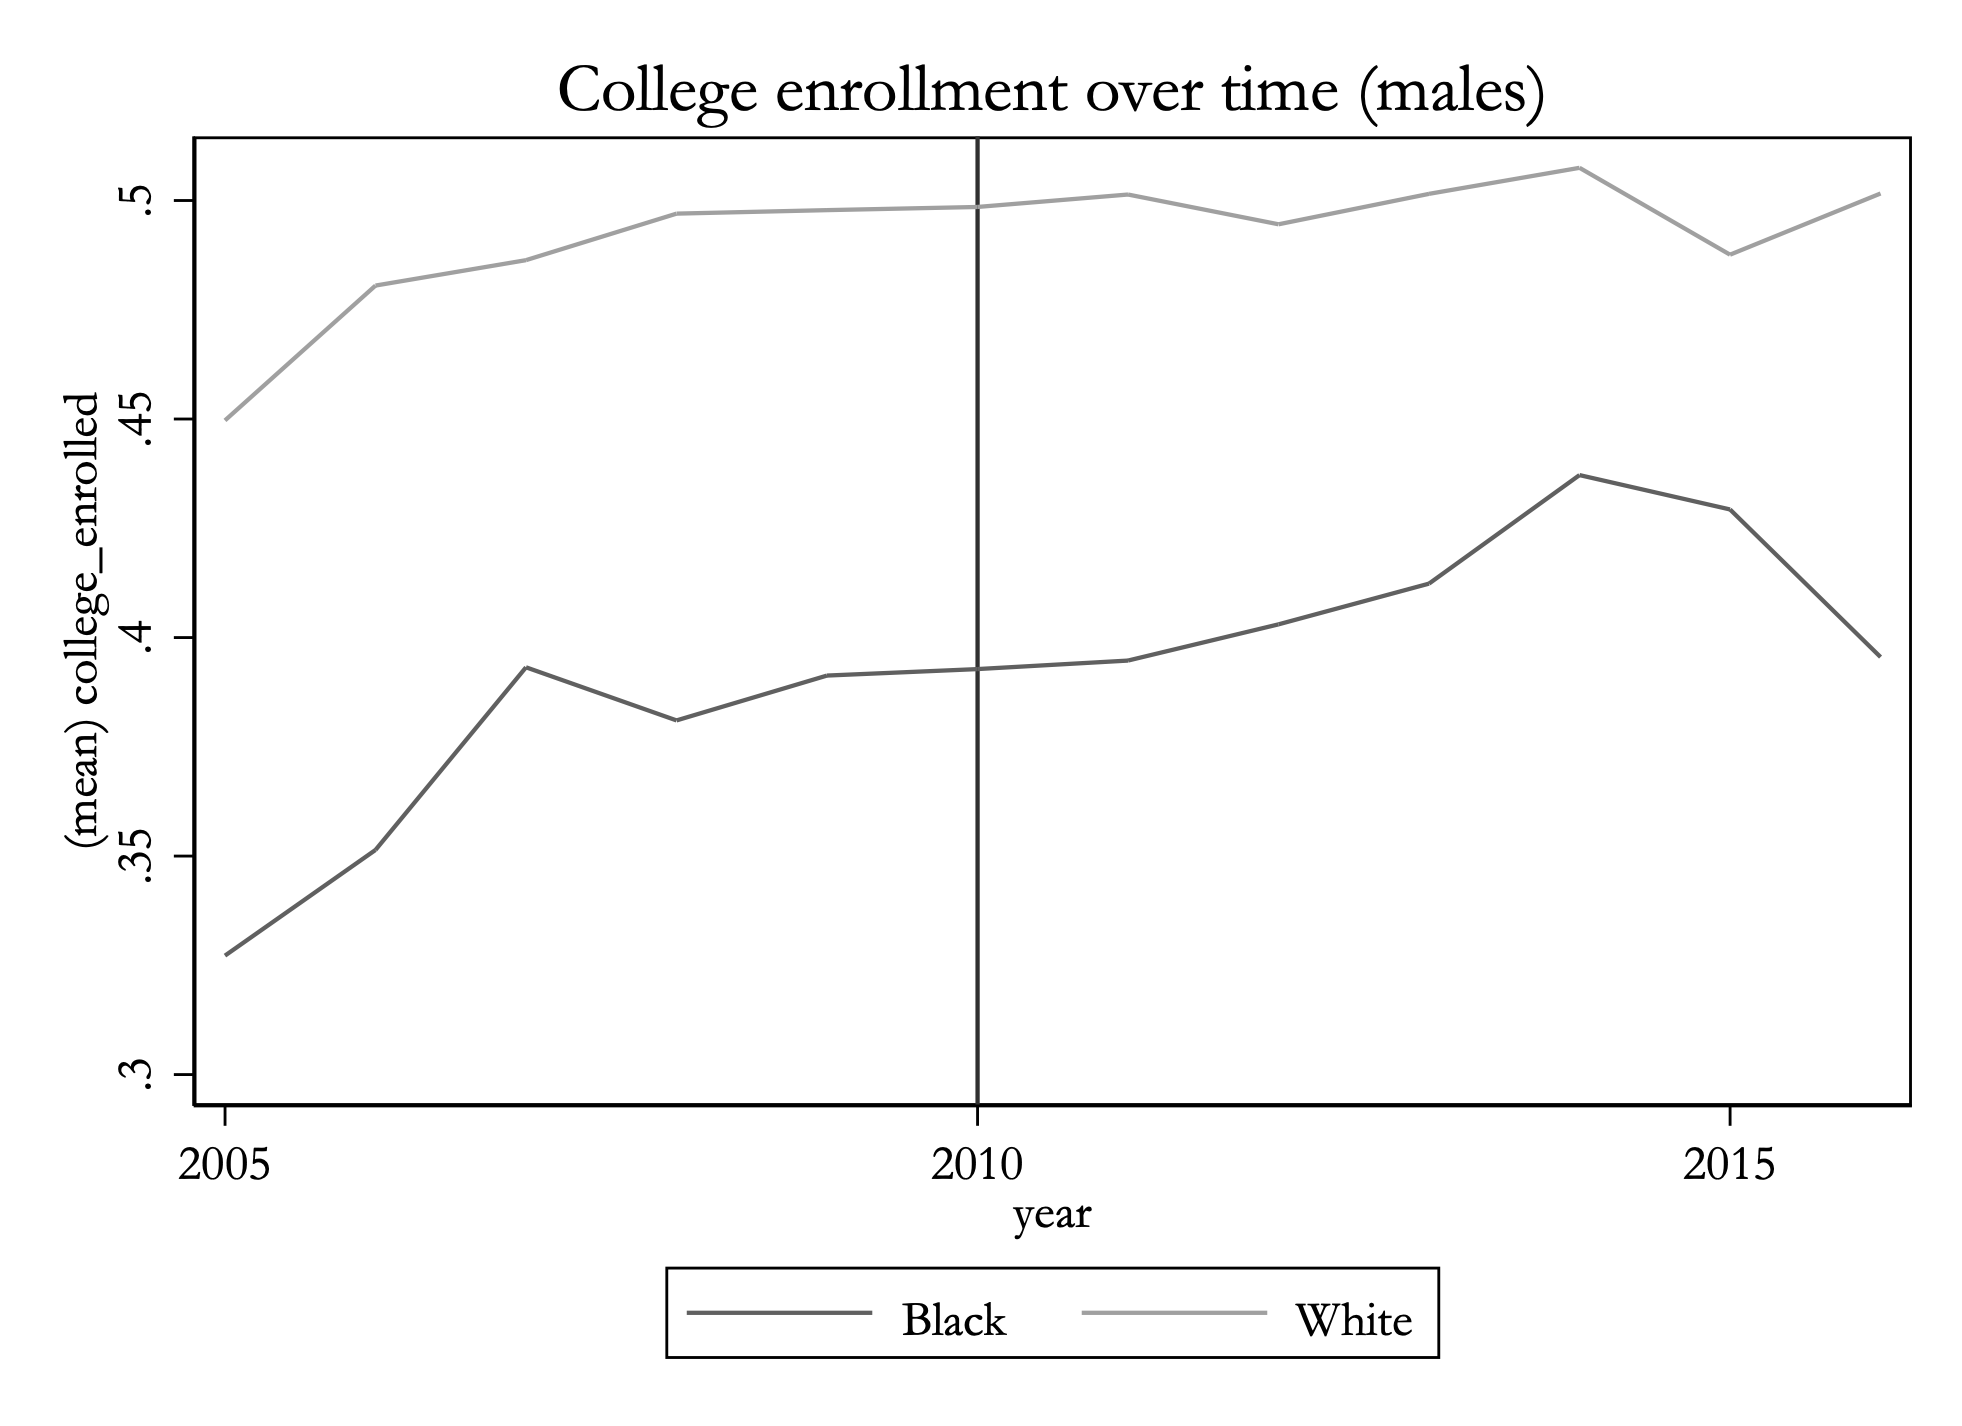
\includegraphics[width=.4\textwidth]{pretrends/2010/college_enroll_byrace_2010.png}
  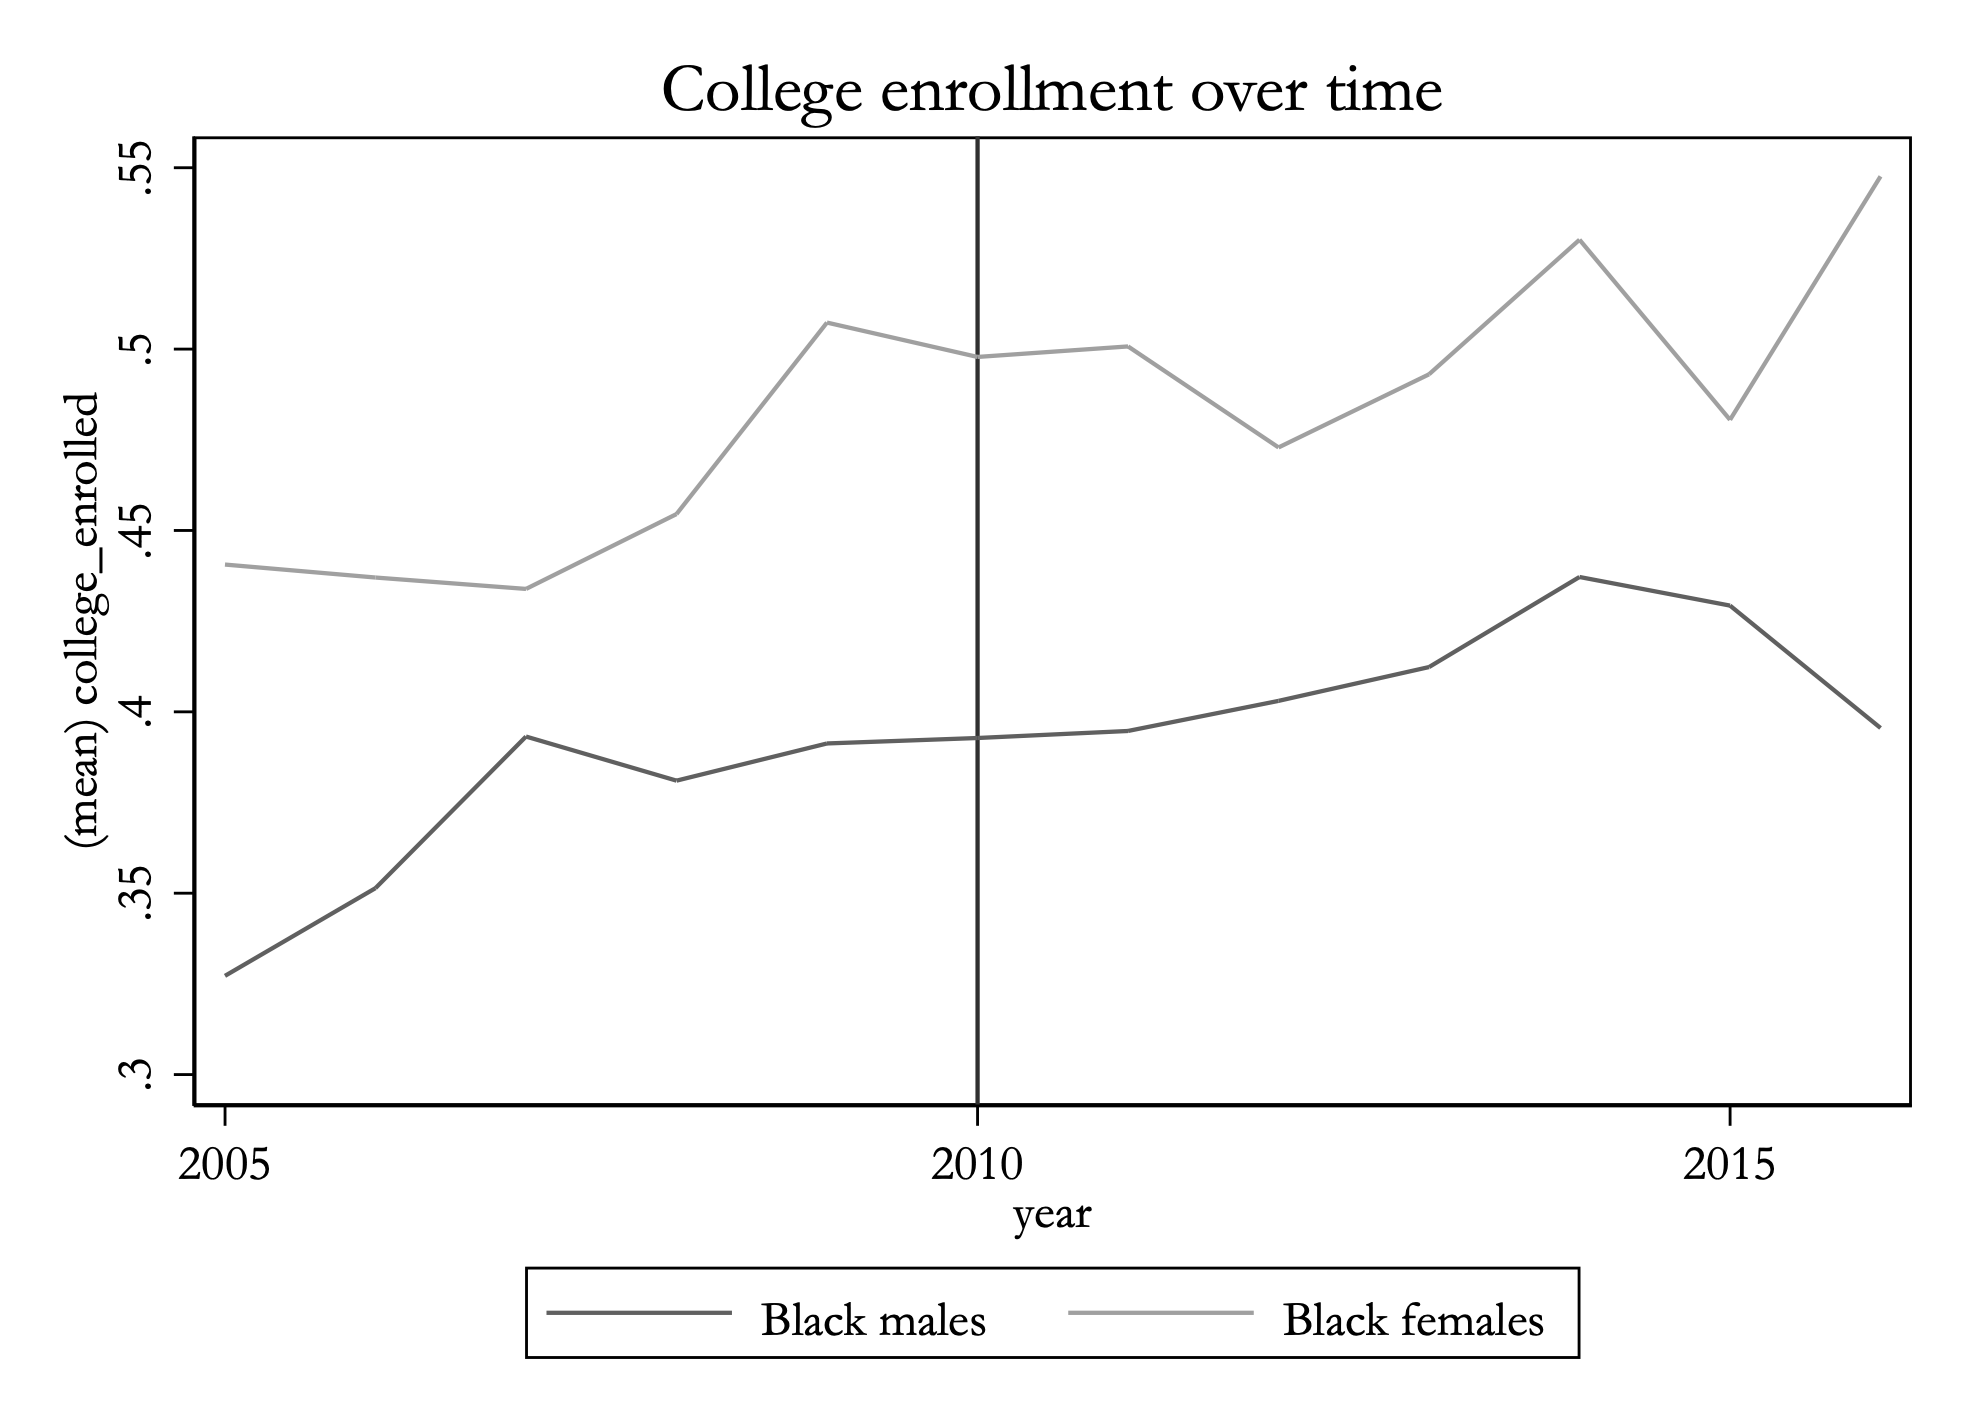
\includegraphics[width=.4\textwidth]{pretrends/2010/college_enroll_bysex_2010.png}
\end{center}

\clearpage

\begin{center}
  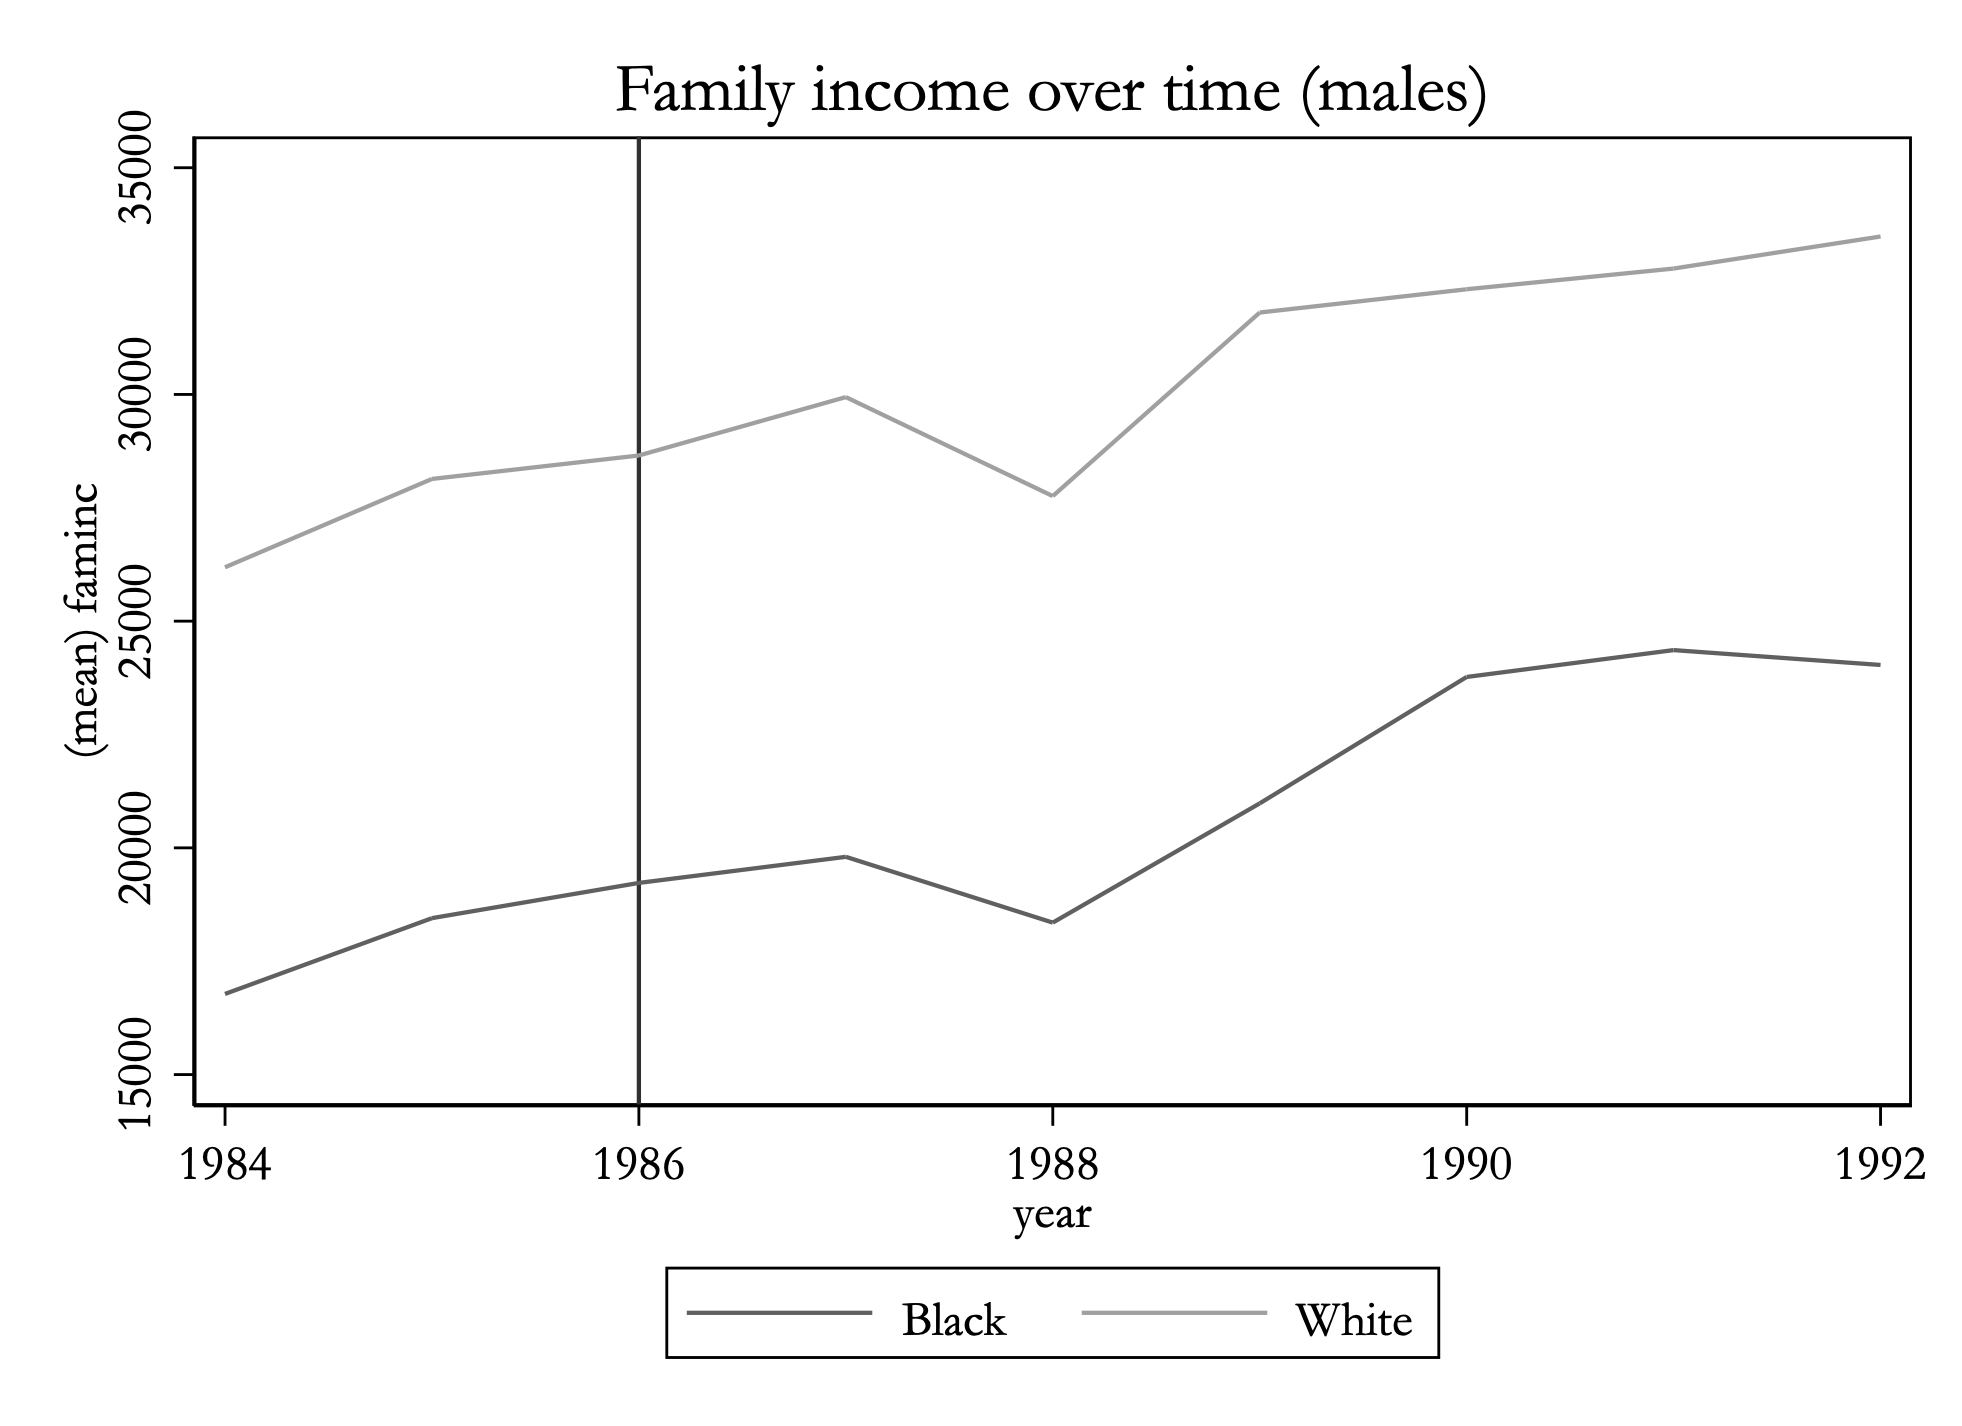
\includegraphics[width=.4\textwidth]{pretrends/1986/faminc_byrace_1986.png}
  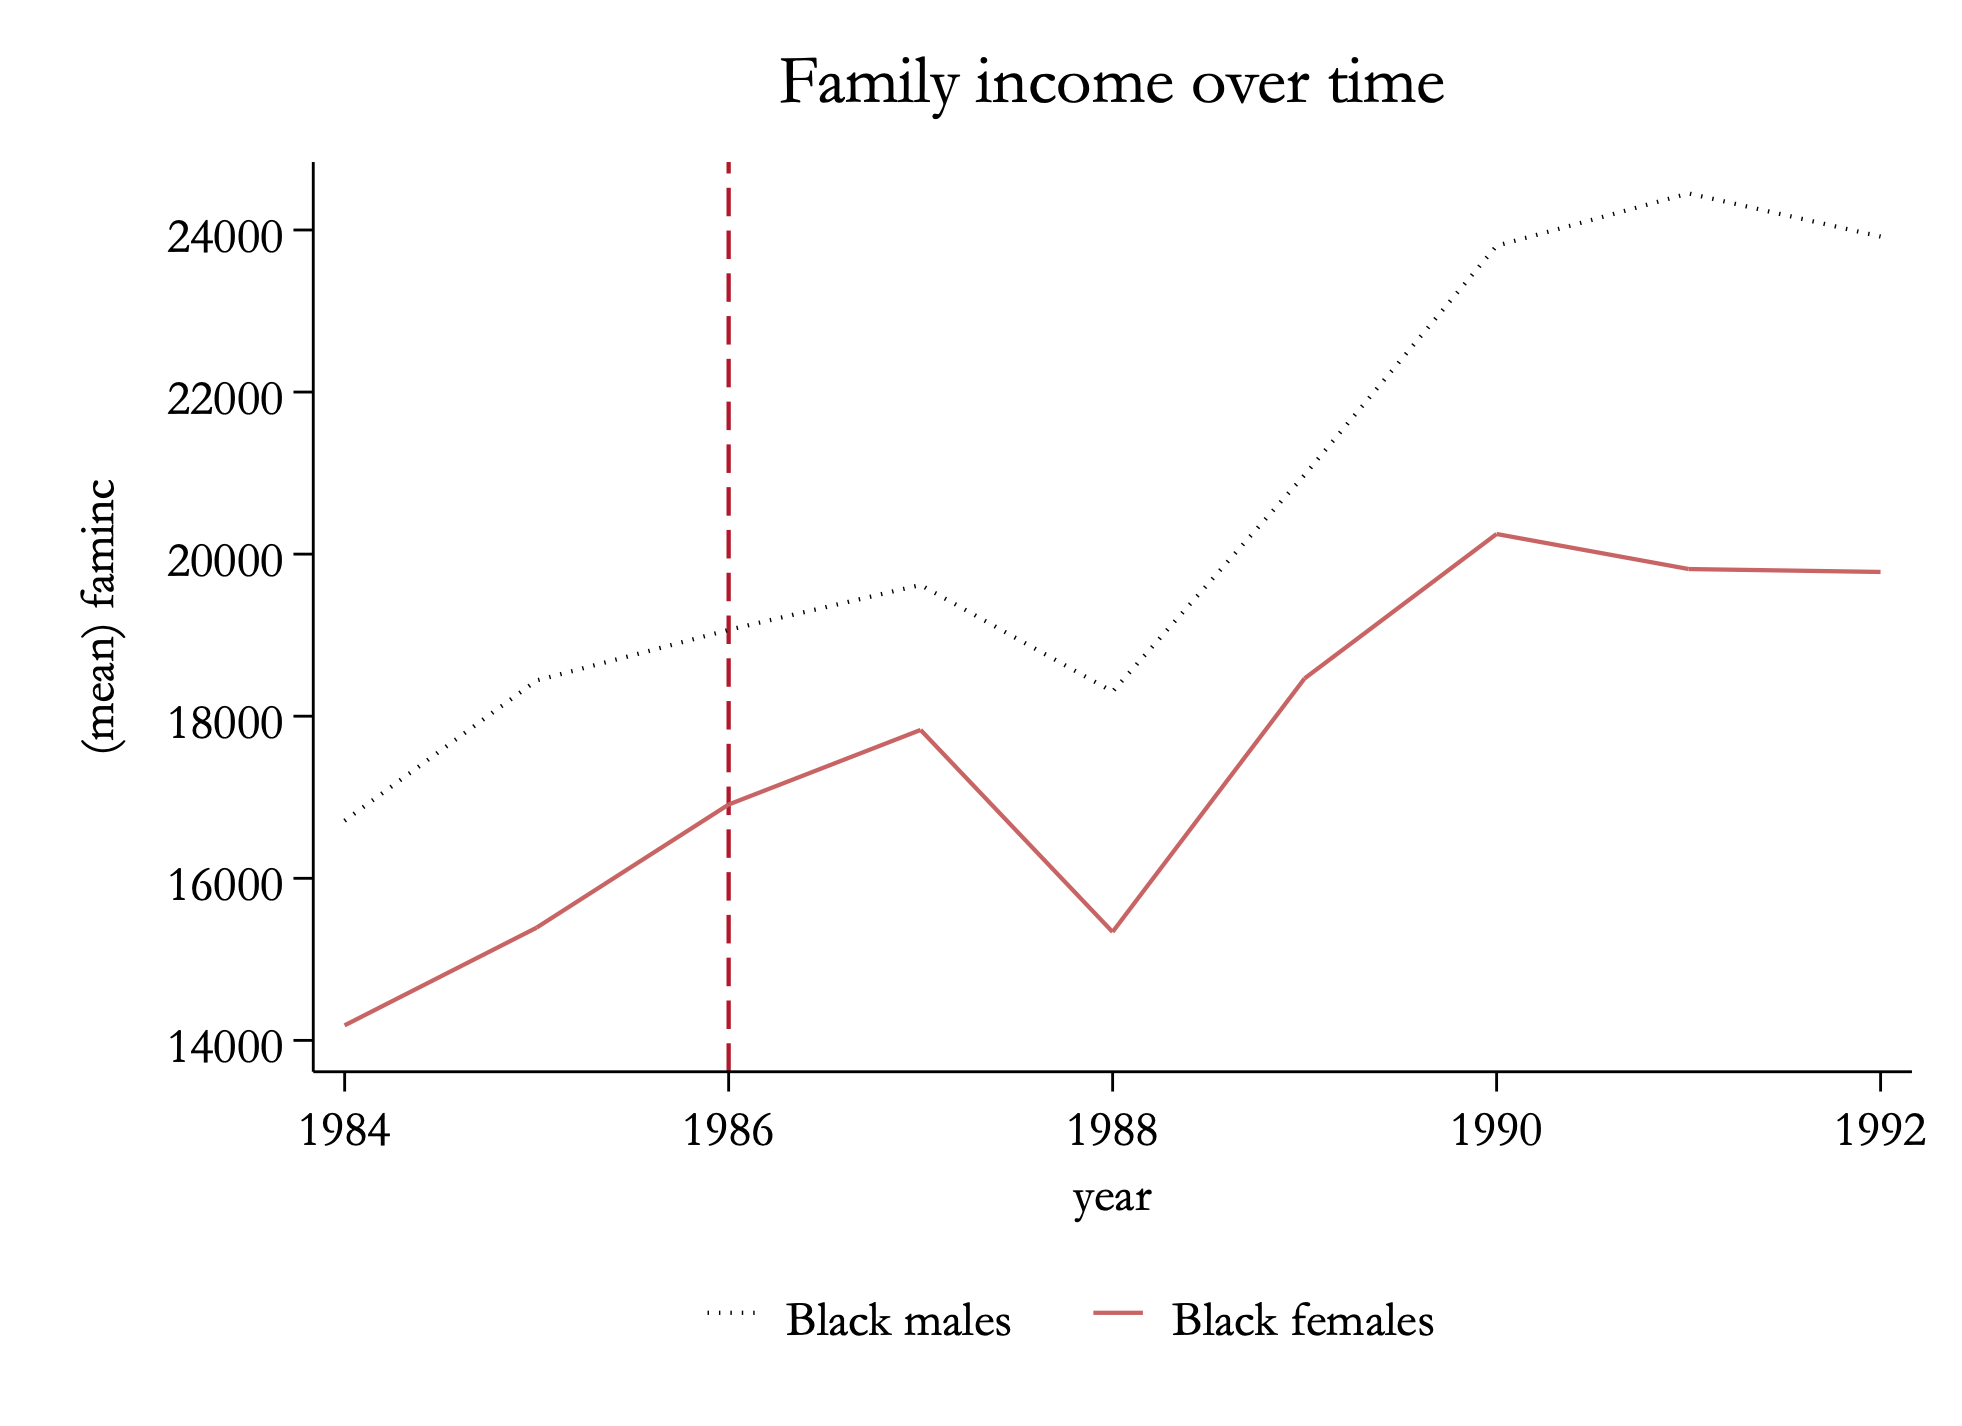
\includegraphics[width=.4\textwidth]{pretrends/1986/faminc_bysex_1986.png}
  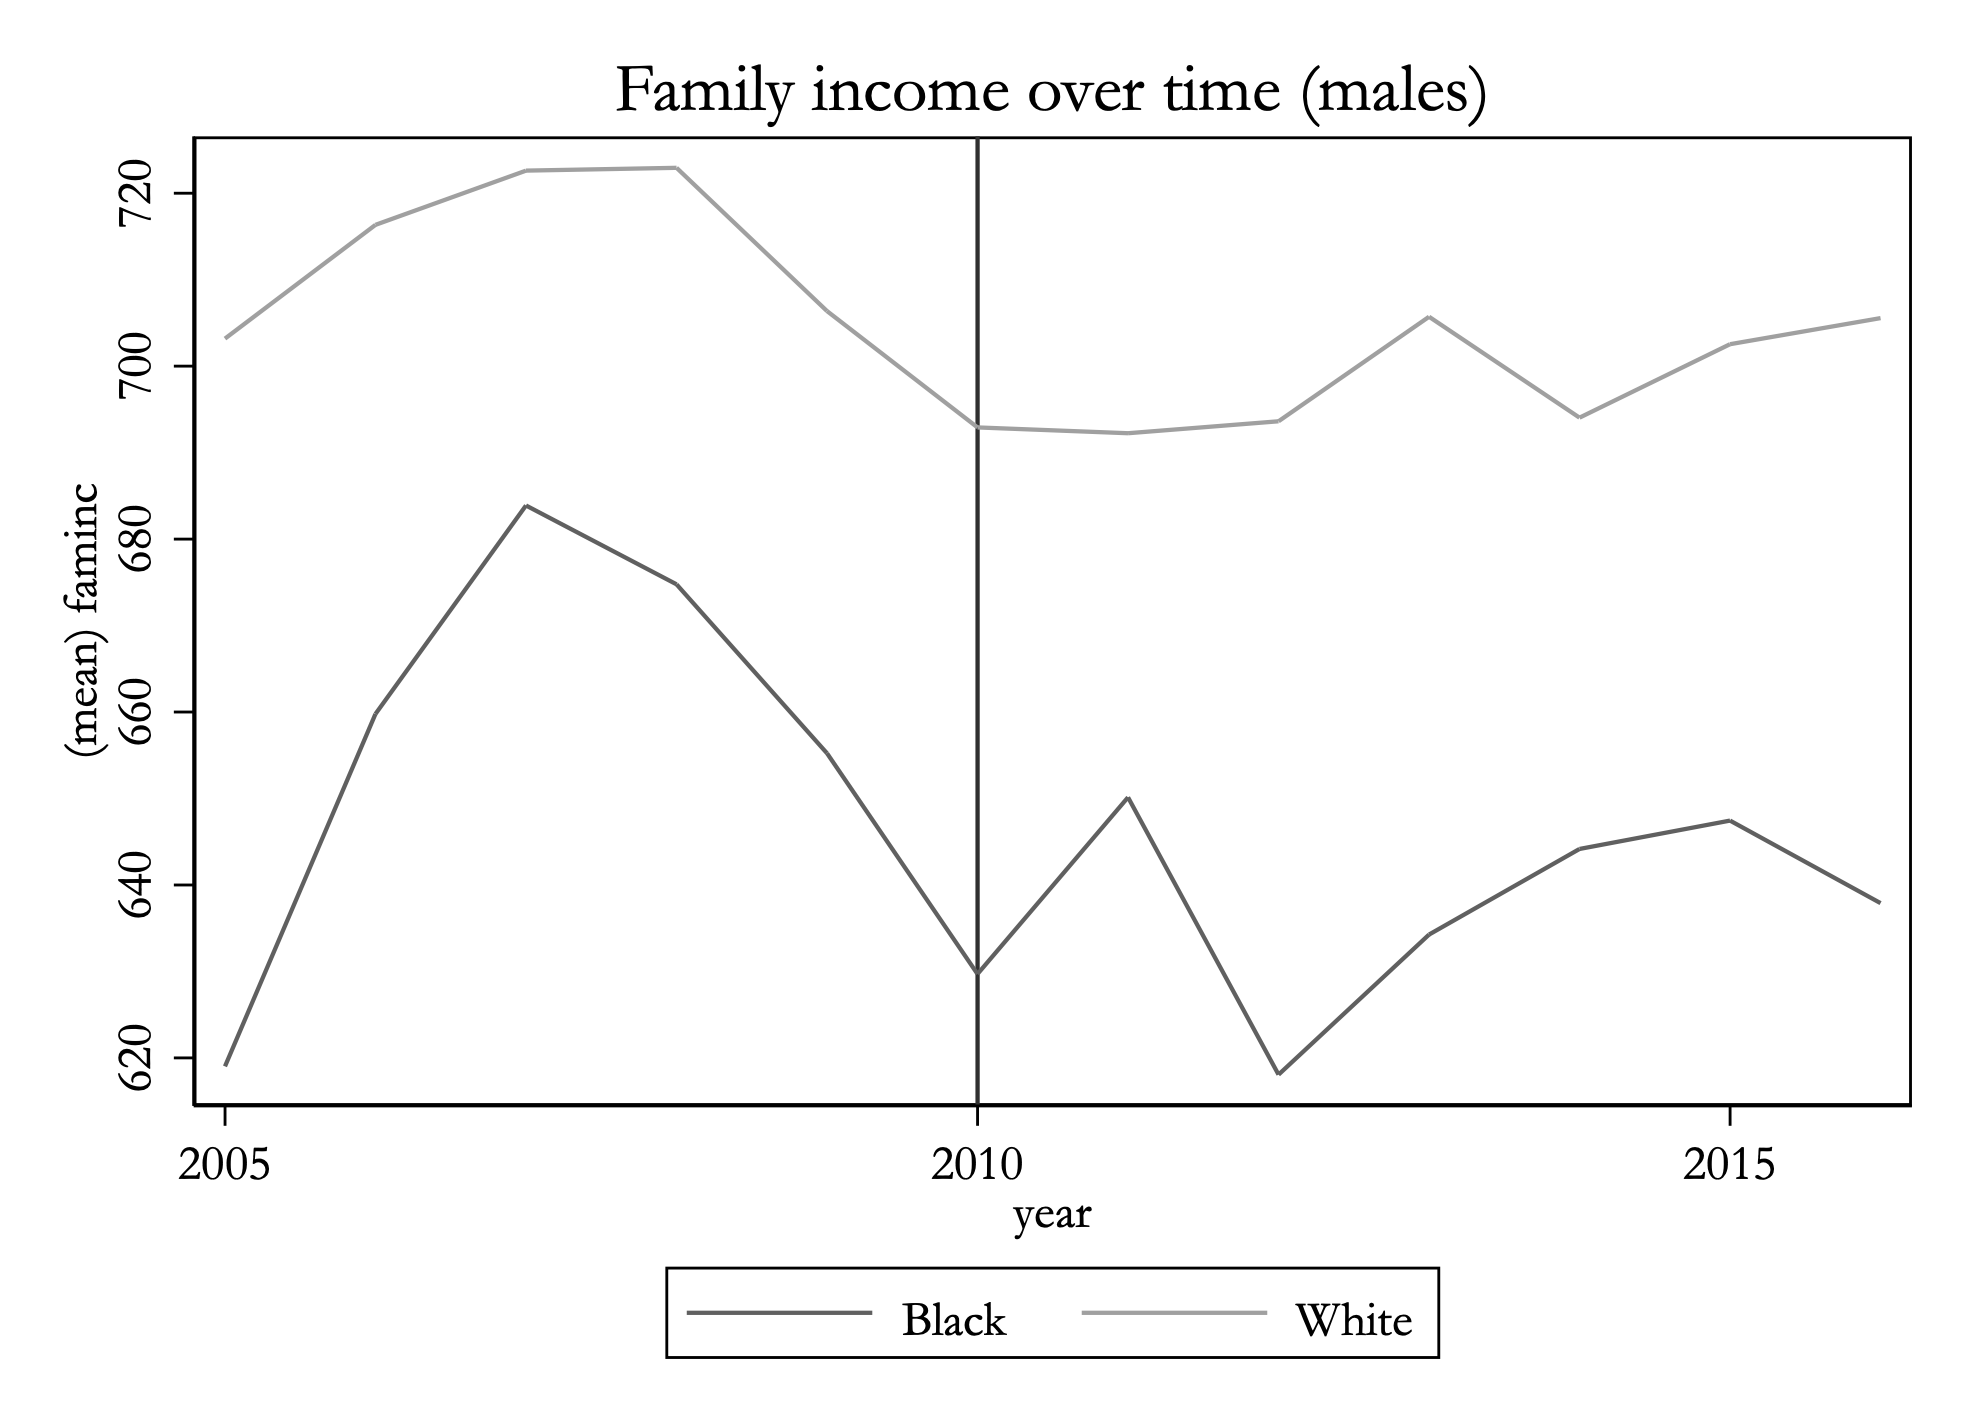
\includegraphics[width=.4\textwidth]{pretrends/2010/faminc_byrace_2010.png}
  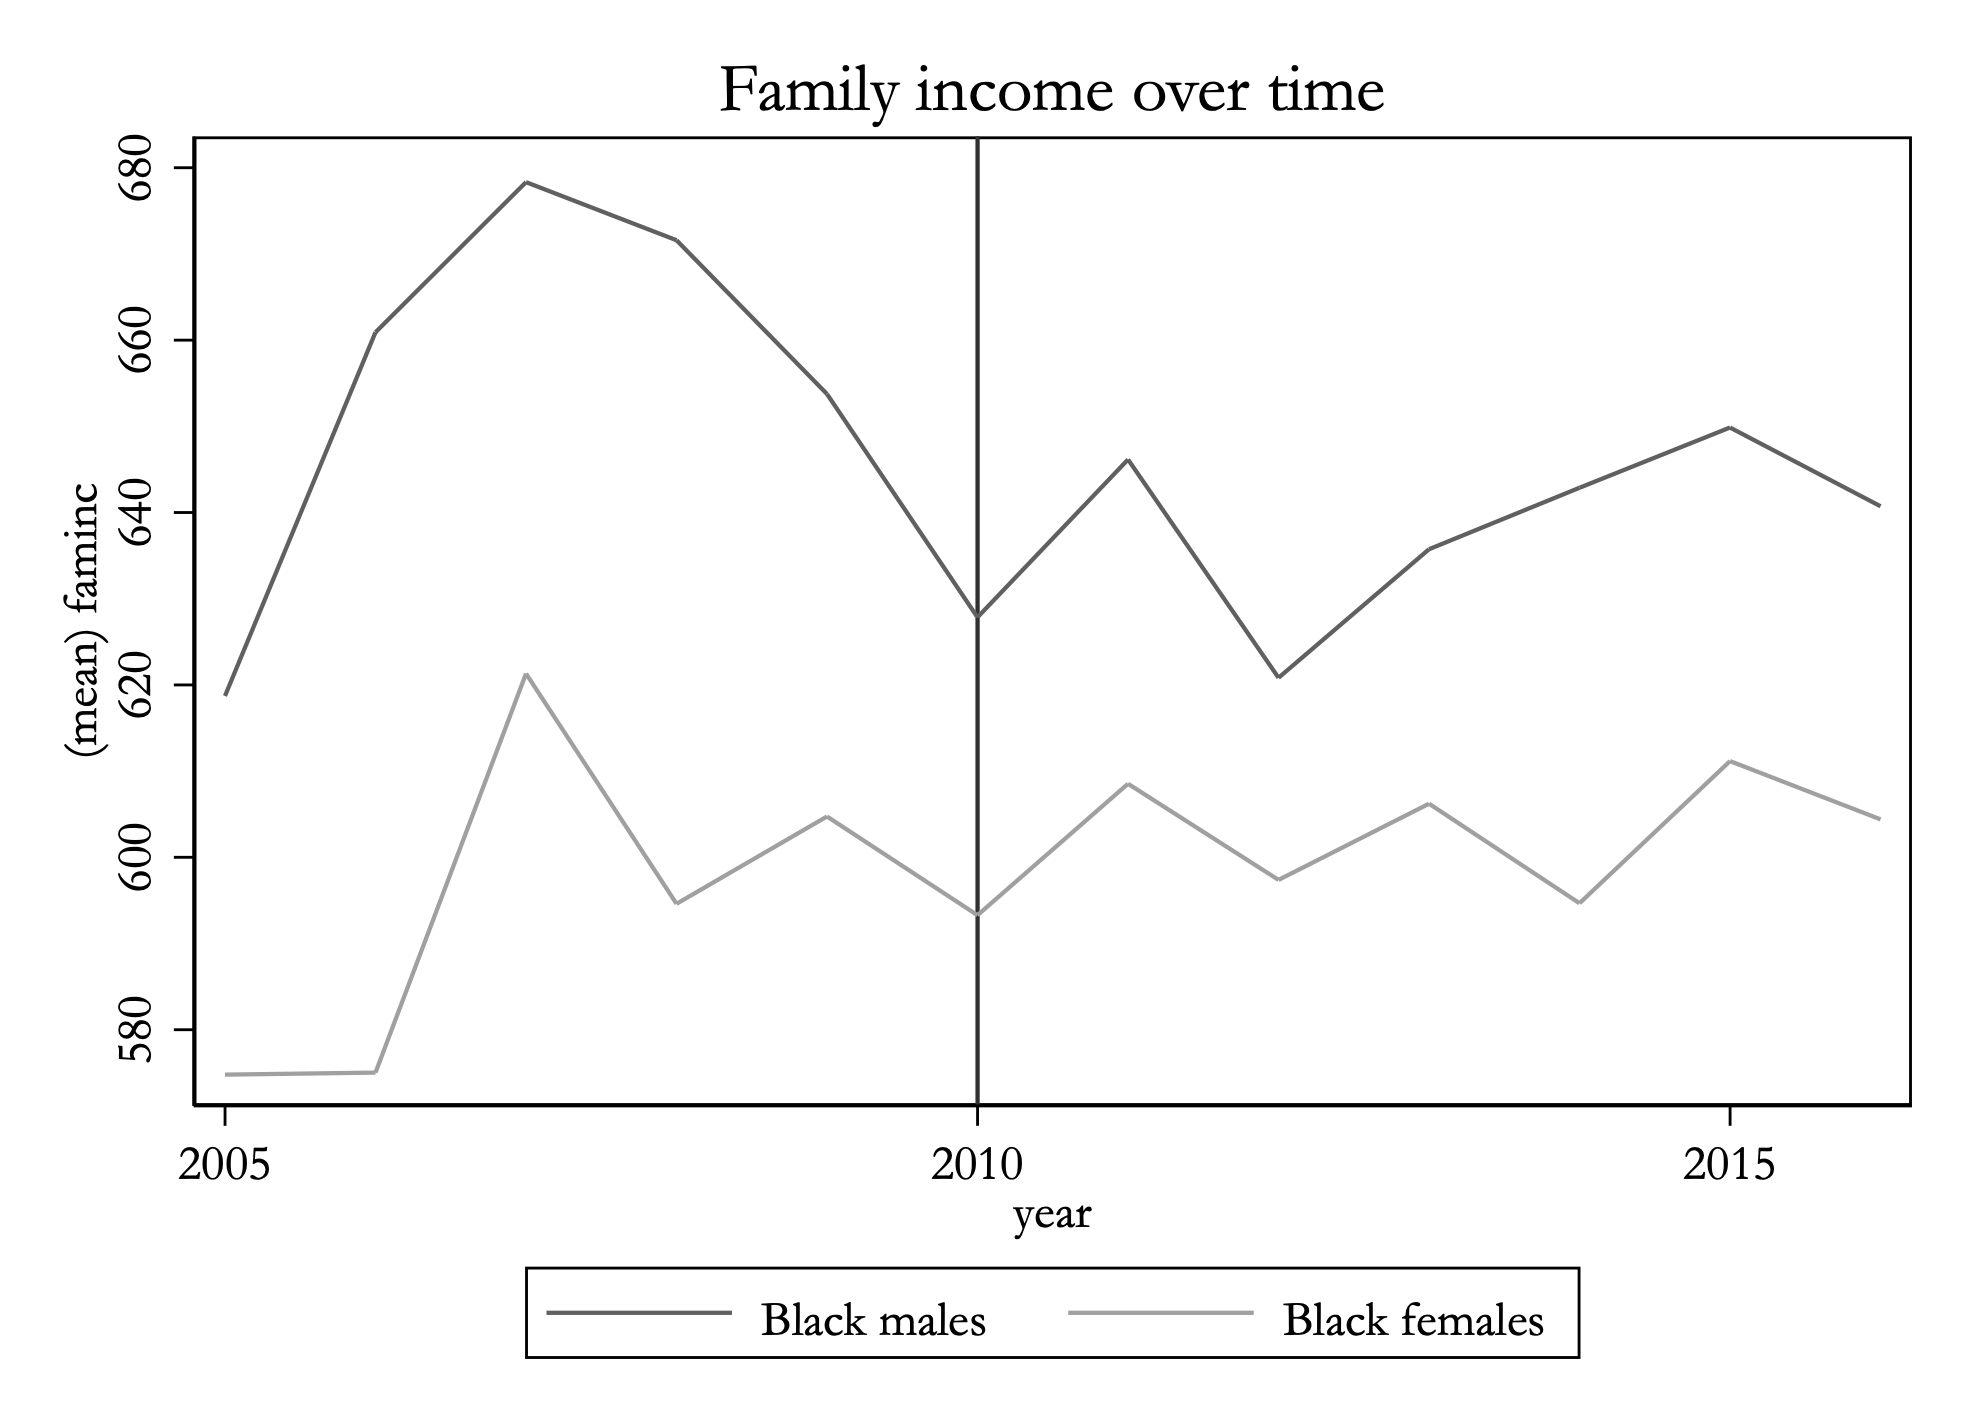
\includegraphics[width=.4\textwidth]{pretrends/2010/faminc_bysex_2010.png}
\end{center}

\clearpage

\begin{figure}[h]
  \caption{College enrollment overtime 1986}
  \centering
  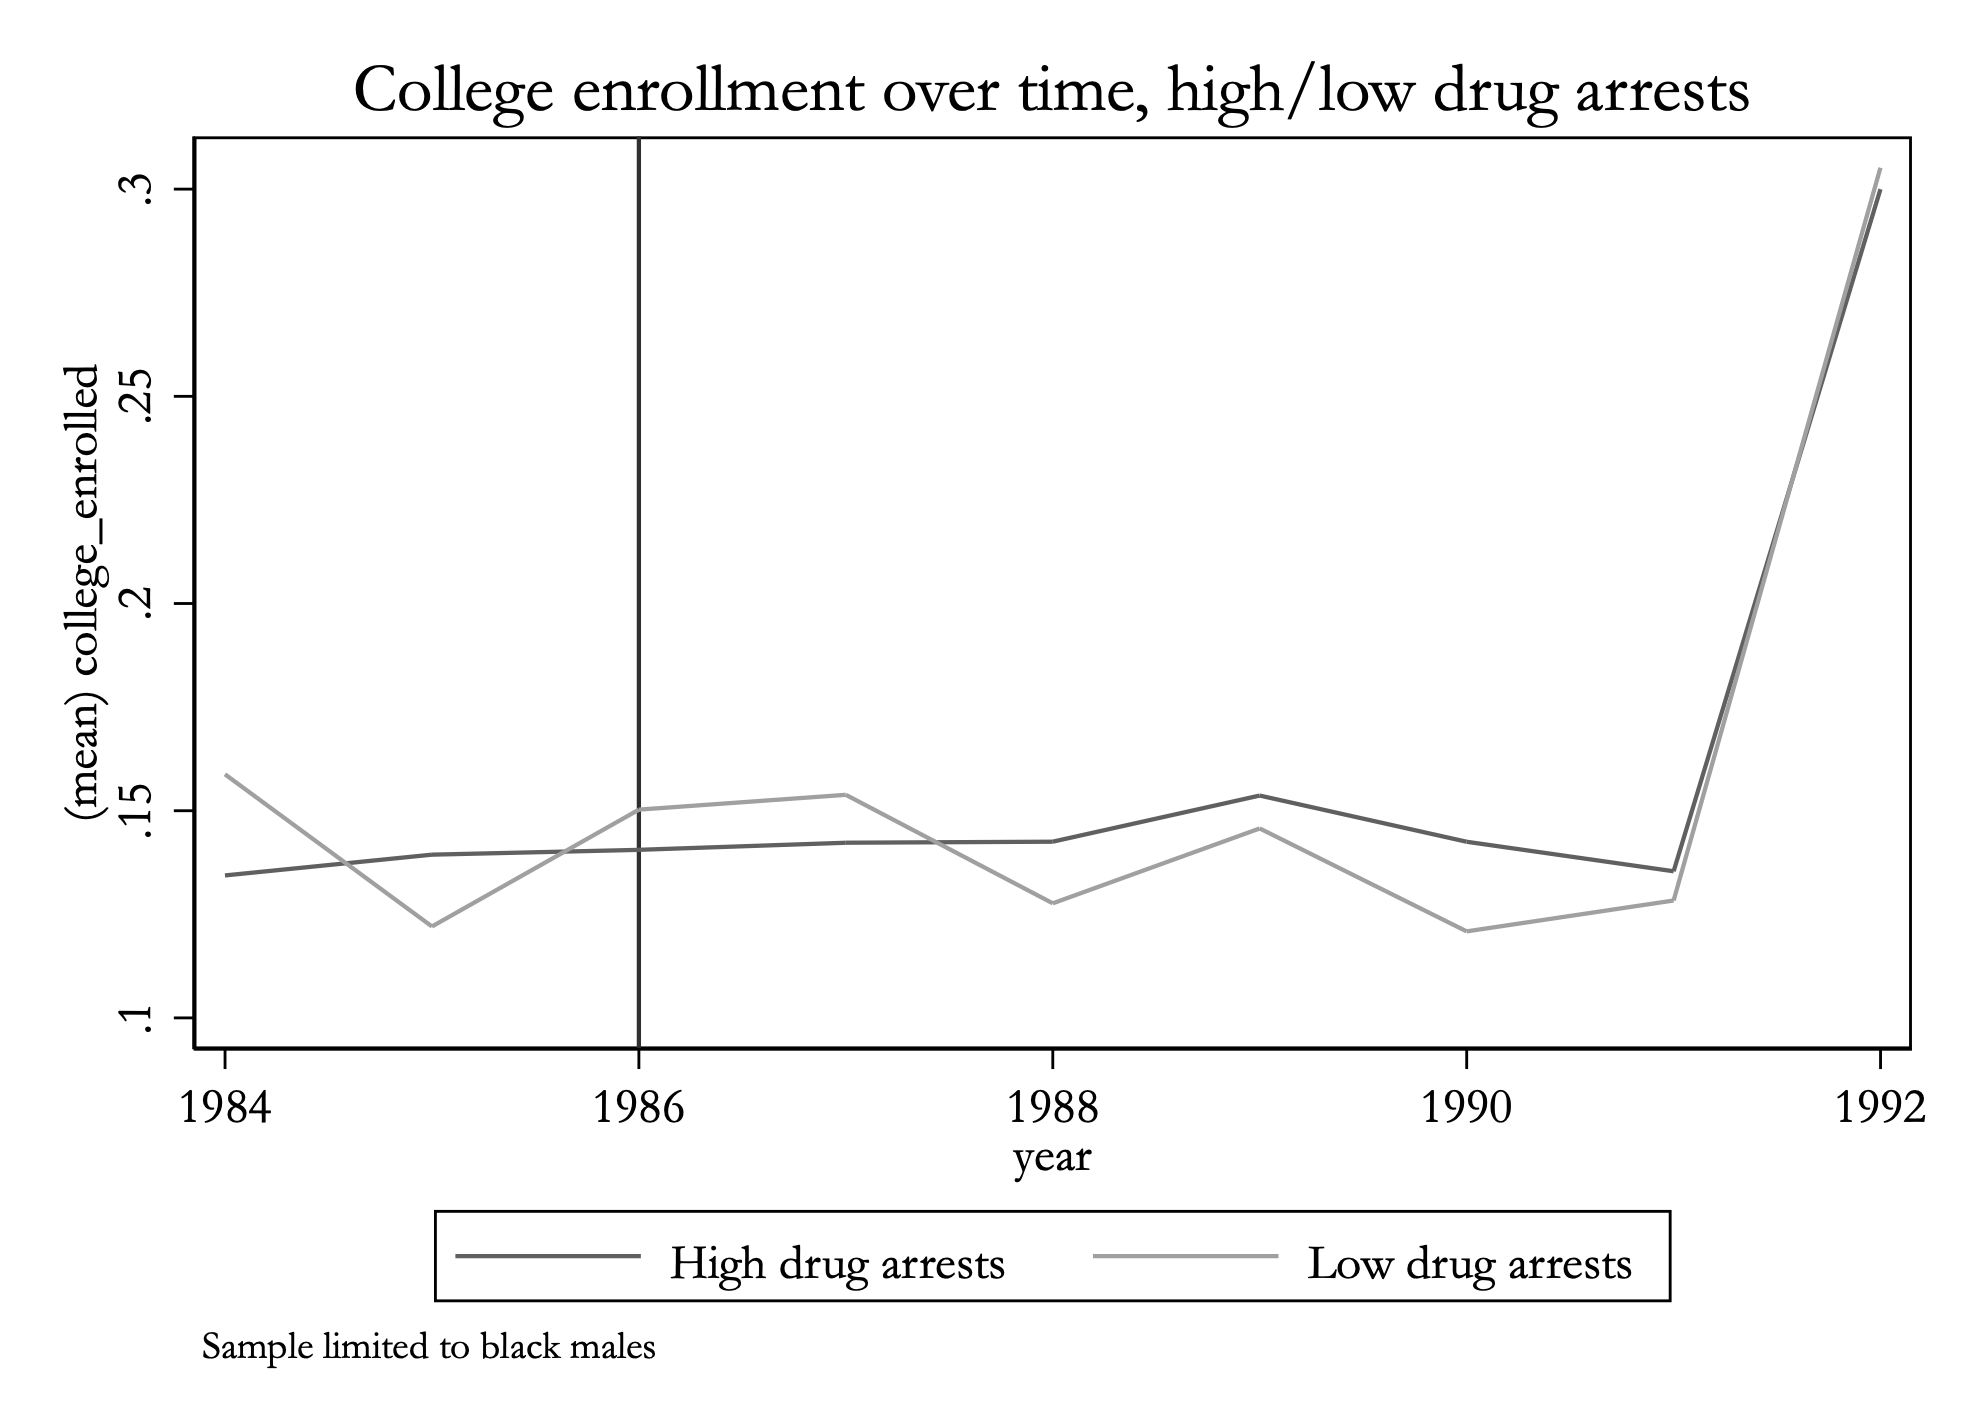
\includegraphics[width=1\textwidth]{pretrends/1986/college_enroll_bydrugarrests_1986.png}
  \label{fig:TBD}
\end{figure}

\clearpage

\begin{figure}[h]
  \caption{College enrollment overtime 2010}
  \centering
  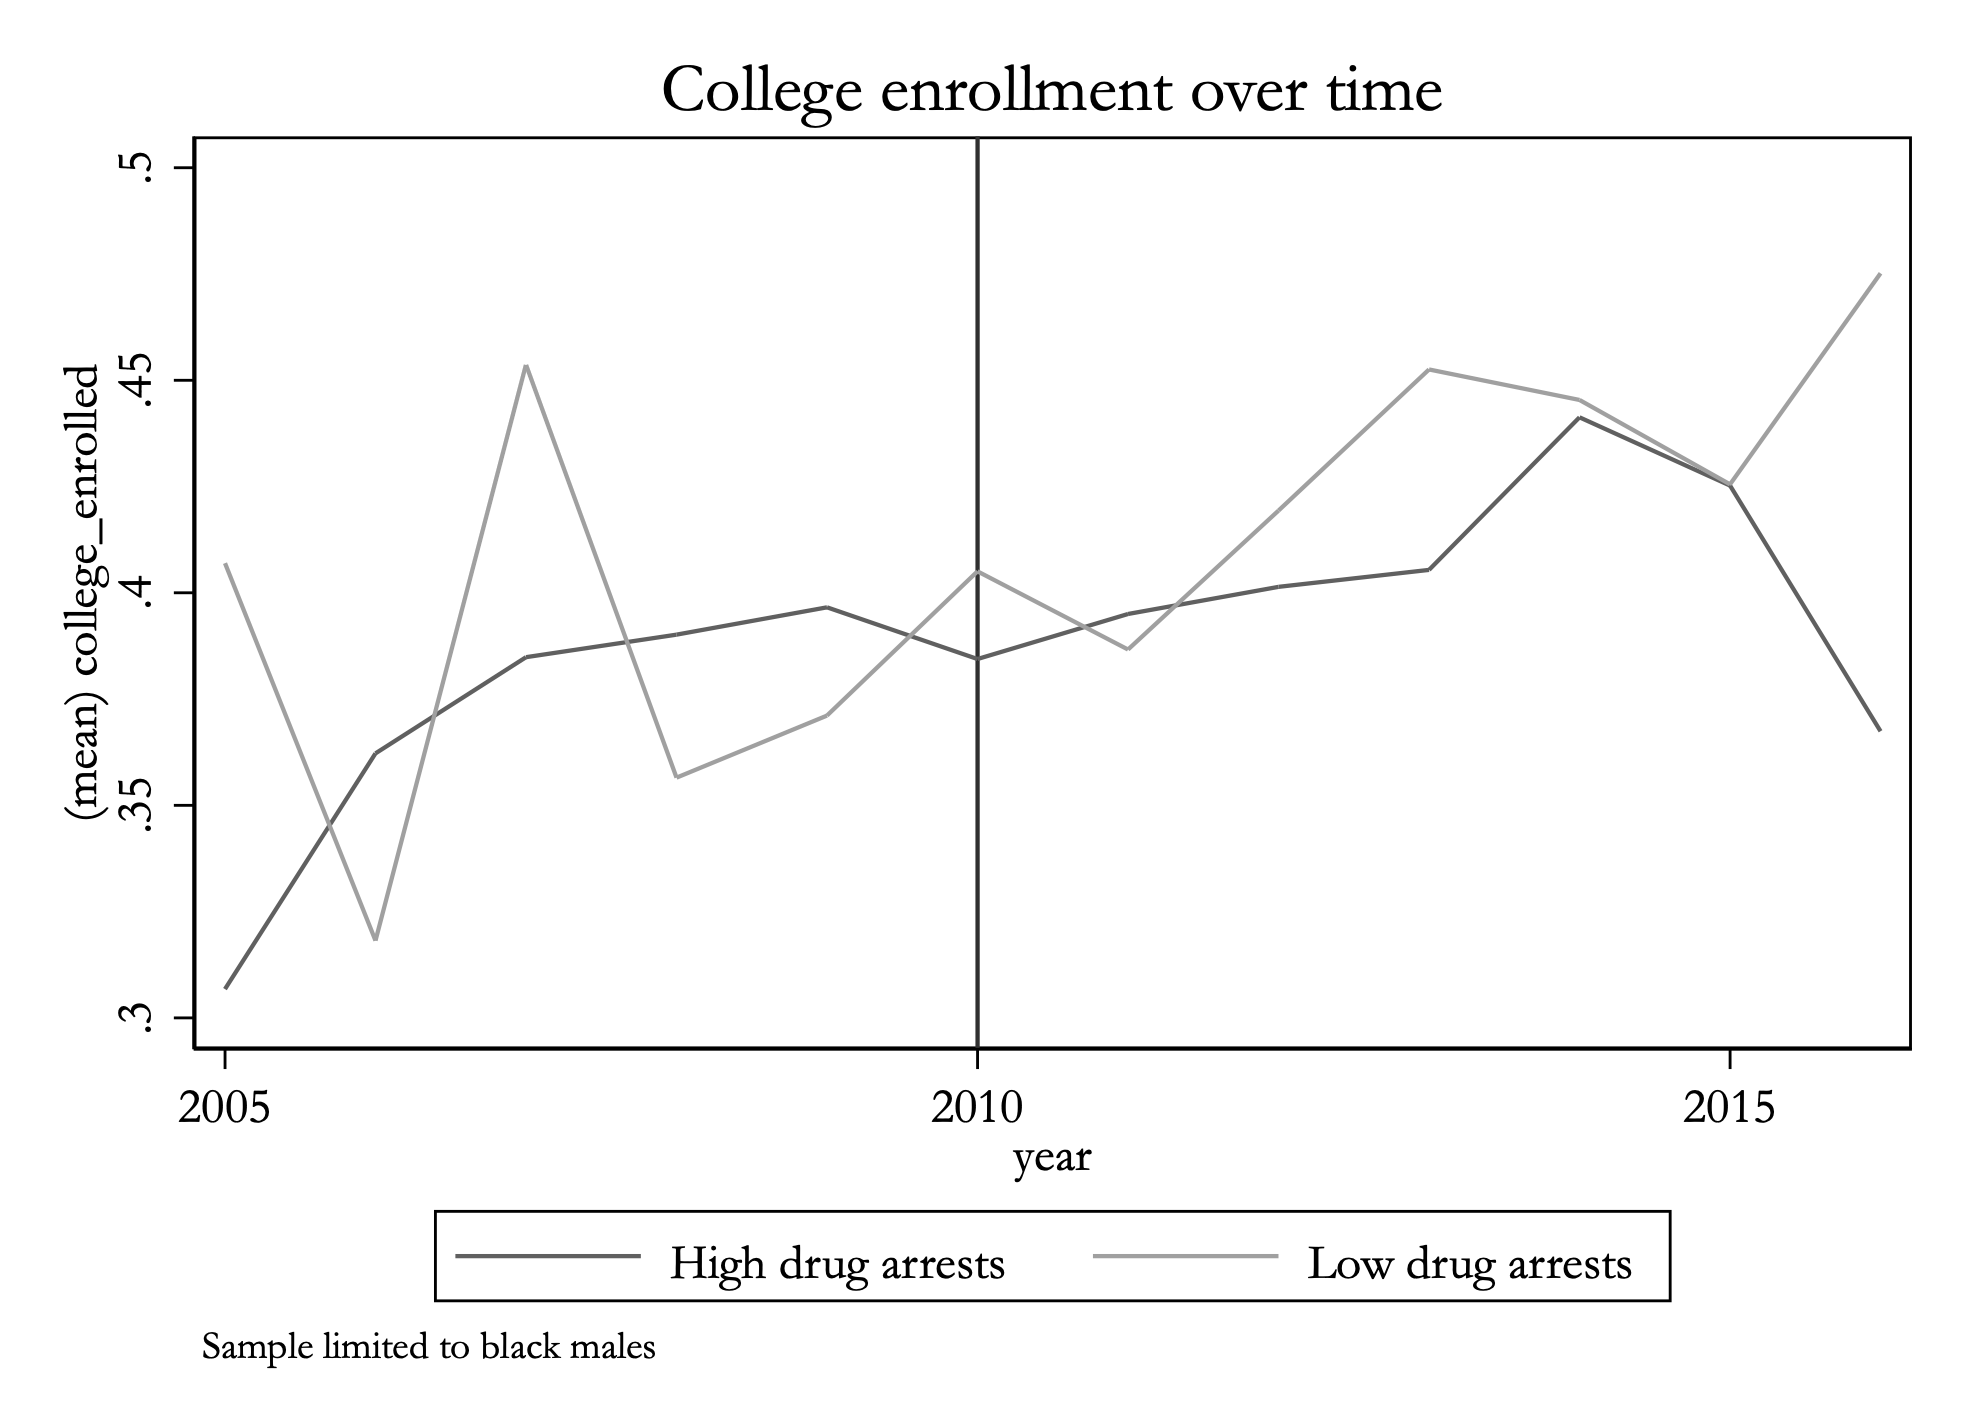
\includegraphics[width=1\textwidth]{pretrends/2010/college_enroll_bydrugarrests_2010.png}
  \label{fig:TBD}
\end{figure}

\clearpage

\begin{figure}[h]
  \caption{Event study 1986, AB arrest rate 18F}
  \centering
  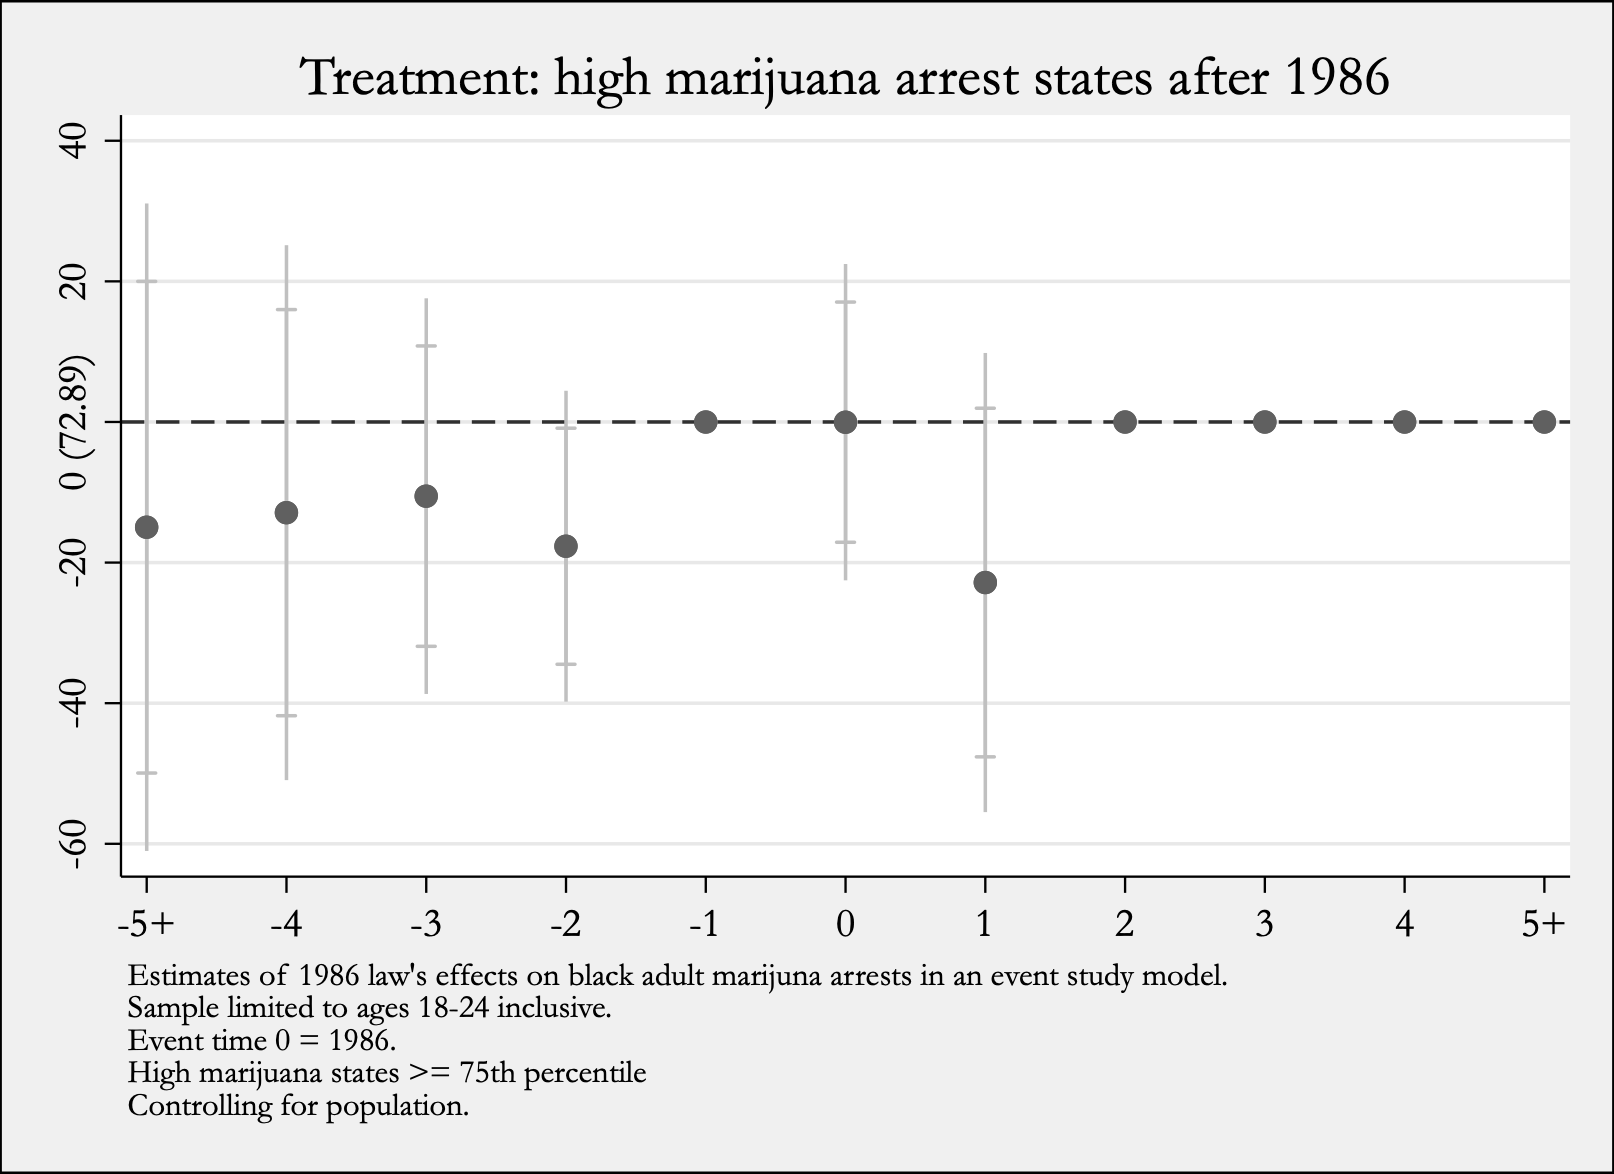
\includegraphics[width=1\textwidth]{eventstudy/high_drug_use/high_marijuana_eventstudy_1986.png}
  \label{fig:TBD}
\end{figure}

\begin{figure*}[h]
  \caption{Pretrends for Event study 1986, AB arrest rate 18F}
  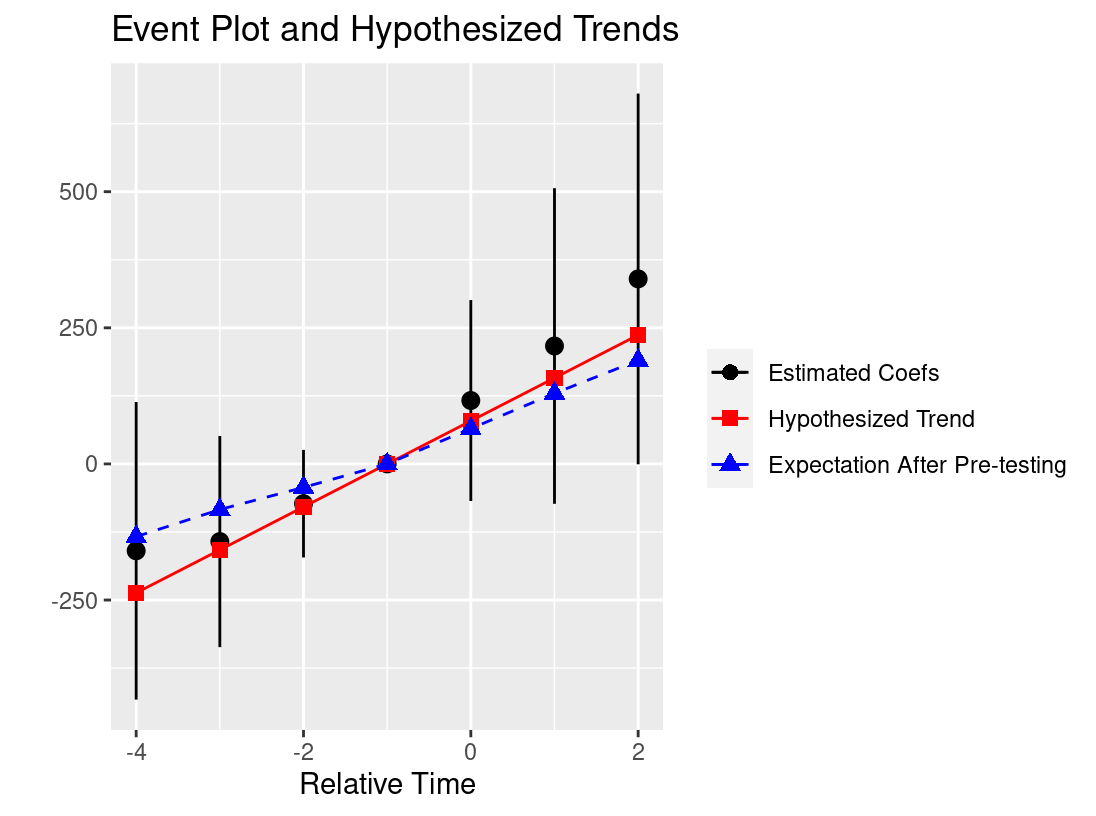
\includegraphics[width=1\textwidth]{roth_test.png}
\end{figure*}

Power: 0.499. Bayes.Factor: 0.550.  Likelihood.Ratio: 2.024

\clearpage

\begin{figure}[h]
  \caption{Event study 2010, AB arrest rate 18F}
  \centering
  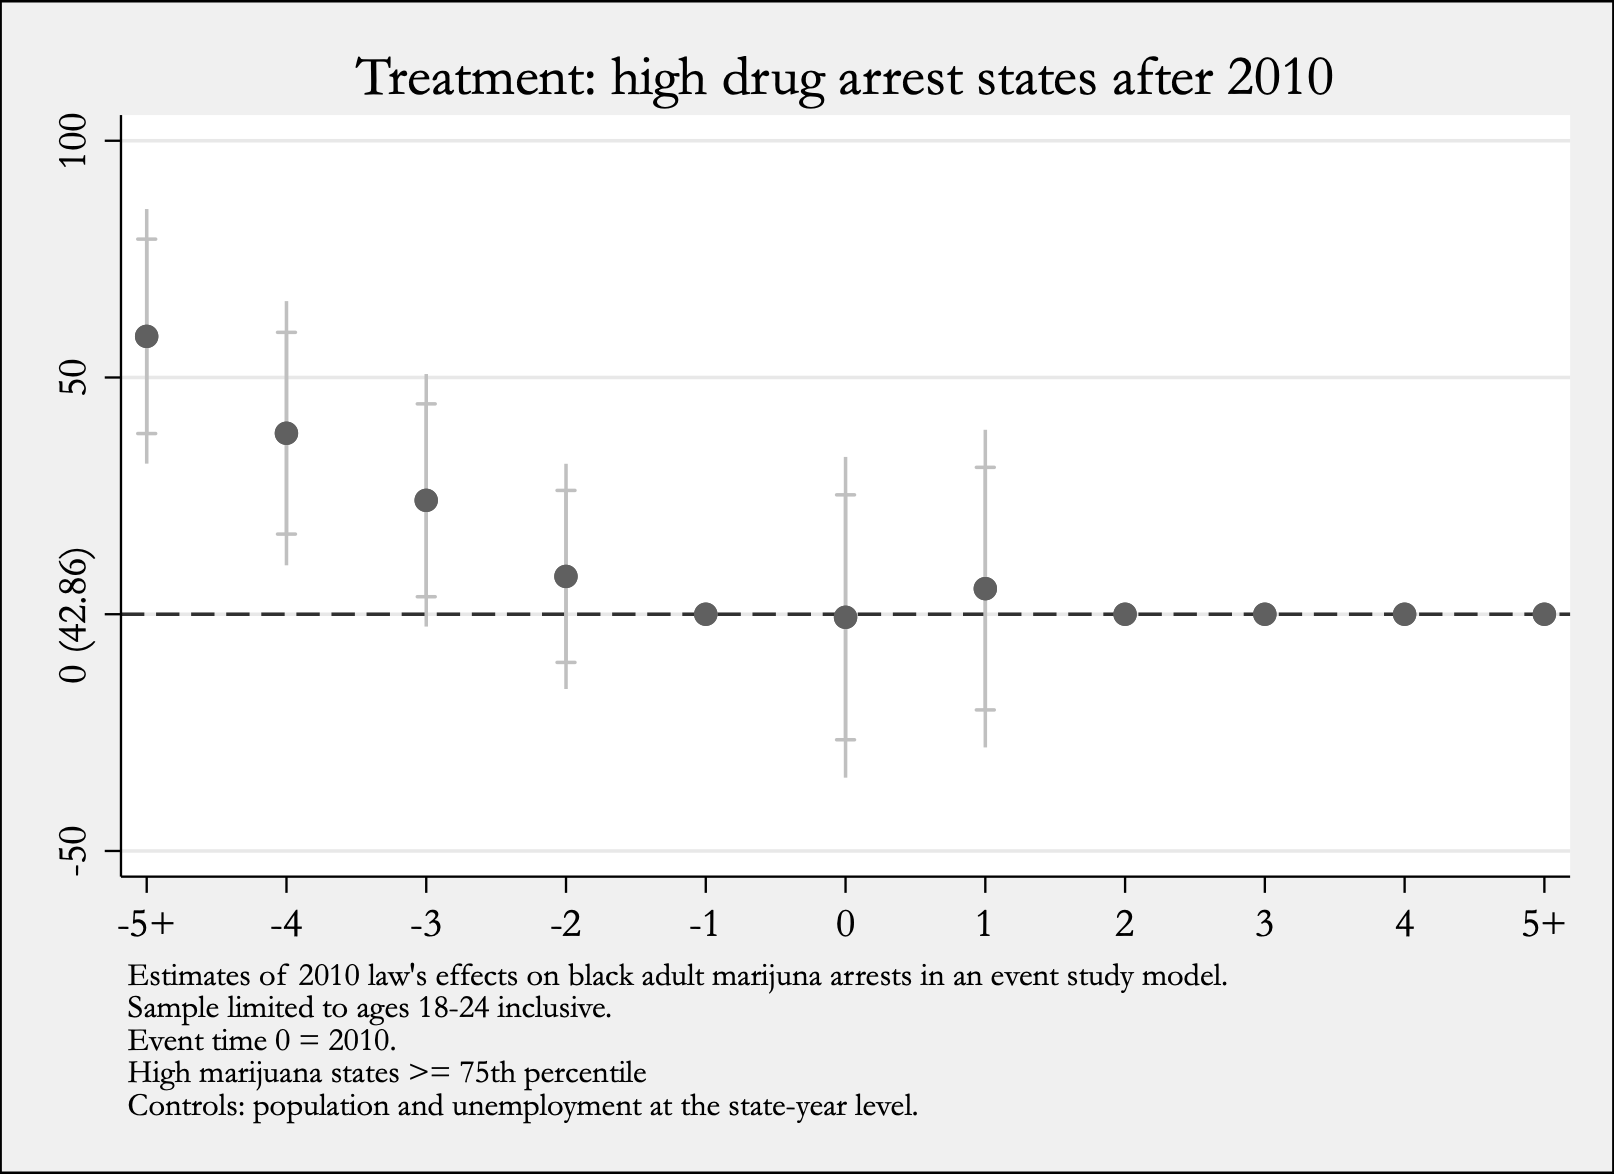
\includegraphics[width=1\textwidth]{eventstudy/high_drug_use/high_marijuana_eventstudy_2010.png}
  \label{fig:TBD}
\end{figure}

\clearpage

\begin{figure}[h]
  \caption{Event study 1986, college enrollment 18}
  \centering
  \includegraphics[width=1\textwidth]{eventstudy/black_college_1986.png}
  \label{fig:TBD}
\end{figure}

to be evaluated

%%%%%%%%%%%%%%%%%%%%%%%%TABLES%%%%%%%%%%%%%%%%%%%%%%%%%%%


\import{../../output/tables/summ_stats/}{cps_summ_stats.tex}
\import{../../output/tables/summ_stats/}{ucr_summ_stats.tex}


\import{../../output/tables/}{britton_table2_DiD.tex}
\import{../../output/tables/}{britton_table2_DiD_control_experiment.tex}

\import{../../output/tables/}{britton_table3_DiD.tex}
\import{../../output/tables/}{britton_table3_DiD_control_experiment.tex}

\import{../../output/tables/}{fair_sentencing_DiD_t1.tex}
\import{../../output/tables/}{fair_sentencing_DiD_t1_control_experiment.tex}

\import{../../output/tables/}{fair_sentencing_DiD_t2.tex}
\import{../../output/tables/}{fair_sentencing_DiD_t2_control_experiment.tex}

\import{../../output/tables/}{DiD_1986_high_low.tex}

\import{../../output/tables/}{ddd_1986.tex}

\import{../../output/tables/}{ddiv_show.tex}


\end{document}
